\documentclass[twoside]{book}

% Packages required by doxygen
\usepackage{fixltx2e}
\usepackage{calc}
\usepackage{doxygen}
\usepackage[export]{adjustbox} % also loads graphicx
\usepackage{graphicx}
\usepackage[utf8]{inputenc}
\usepackage{makeidx}
\usepackage{multicol}
\usepackage{multirow}
\PassOptionsToPackage{warn}{textcomp}
\usepackage{textcomp}
\usepackage[nointegrals]{wasysym}
\usepackage[table]{xcolor}

% Font selection
\usepackage[T1]{fontenc}
\usepackage[scaled=.90]{helvet}
\usepackage{courier}
\usepackage{amssymb}
\usepackage{sectsty}
\renewcommand{\familydefault}{\sfdefault}
\allsectionsfont{%
  \fontseries{bc}\selectfont%
  \color{darkgray}%
}
\renewcommand{\DoxyLabelFont}{%
  \fontseries{bc}\selectfont%
  \color{darkgray}%
}
\newcommand{\+}{\discretionary{\mbox{\scriptsize$\hookleftarrow$}}{}{}}

% Page & text layout
\usepackage{geometry}
\geometry{%
  a4paper,%
  top=2.5cm,%
  bottom=2.5cm,%
  left=2.5cm,%
  right=2.5cm%
}
\tolerance=750
\hfuzz=15pt
\hbadness=750
\setlength{\emergencystretch}{15pt}
\setlength{\parindent}{0cm}
\setlength{\parskip}{3ex plus 2ex minus 2ex}
\makeatletter
\renewcommand{\paragraph}{%
  \@startsection{paragraph}{4}{0ex}{-1.0ex}{1.0ex}{%
    \normalfont\normalsize\bfseries\SS@parafont%
  }%
}
\renewcommand{\subparagraph}{%
  \@startsection{subparagraph}{5}{0ex}{-1.0ex}{1.0ex}{%
    \normalfont\normalsize\bfseries\SS@subparafont%
  }%
}
\makeatother

% Headers & footers
\usepackage{fancyhdr}
\pagestyle{fancyplain}
\fancyhead[LE]{\fancyplain{}{\bfseries\thepage}}
\fancyhead[CE]{\fancyplain{}{}}
\fancyhead[RE]{\fancyplain{}{\bfseries\leftmark}}
\fancyhead[LO]{\fancyplain{}{\bfseries\rightmark}}
\fancyhead[CO]{\fancyplain{}{}}
\fancyhead[RO]{\fancyplain{}{\bfseries\thepage}}
\fancyfoot[LE]{\fancyplain{}{}}
\fancyfoot[CE]{\fancyplain{}{}}
\fancyfoot[RE]{\fancyplain{}{\bfseries\scriptsize Generated by Doxygen }}
\fancyfoot[LO]{\fancyplain{}{\bfseries\scriptsize Generated by Doxygen }}
\fancyfoot[CO]{\fancyplain{}{}}
\fancyfoot[RO]{\fancyplain{}{}}
\renewcommand{\footrulewidth}{0.4pt}
\renewcommand{\chaptermark}[1]{%
  \markboth{#1}{}%
}
\renewcommand{\sectionmark}[1]{%
  \markright{\thesection\ #1}%
}

% Indices & bibliography
\usepackage{natbib}
\usepackage[titles]{tocloft}
\setcounter{tocdepth}{3}
\setcounter{secnumdepth}{5}
\makeindex

% Hyperlinks (required, but should be loaded last)
\usepackage{ifpdf}
\ifpdf
  \usepackage[pdftex,pagebackref=true]{hyperref}
\else
  \usepackage[ps2pdf,pagebackref=true]{hyperref}
\fi
\hypersetup{%
  colorlinks=true,%
  linkcolor=blue,%
  citecolor=blue,%
  unicode%
}

% Custom commands
\newcommand{\clearemptydoublepage}{%
  \newpage{\pagestyle{empty}\cleardoublepage}%
}

\usepackage{caption}
\captionsetup{labelsep=space,justification=centering,font={bf},singlelinecheck=off,skip=4pt,position=top}

%===== C O N T E N T S =====

\begin{document}

% Titlepage & ToC
\hypersetup{pageanchor=false,
             bookmarksnumbered=true,
             pdfencoding=unicode
            }
\pagenumbering{alph}
\begin{titlepage}
\vspace*{7cm}
\begin{center}%
{\Large My Project }\\
\vspace*{1cm}
{\large Generated by Doxygen 1.8.12}\\
\end{center}
\end{titlepage}
\clearemptydoublepage
\pagenumbering{roman}
\tableofcontents
\clearemptydoublepage
\pagenumbering{arabic}
\hypersetup{pageanchor=true}

%--- Begin generated contents ---
\chapter{R\+E\+A\+D\+ME}
\label{md__r_e_a_d_m_e}
\hypertarget{md__r_e_a_d_m_e}{}
i\+Cyber\+Security Inc.

You are to create an on-\/line pamphlet for i\+Cyber\+Security Inc. The company provides methodologies so organizations can detect, respond to, and contain advanced cyber security attacks.

You must implement the vector class as outlined in the \hyperlink{vector_8h_source}{vector.\+h} specification below. Vector will be used to store the i\+Cyber\+Security customer list. Your vector class is a close approximation to the S\+TL vector class. Vector supports the following basic operations\+: constructors for one or more arguments, default constructors, copy constructor, copy assignment, move constructor, move assignment and destructor. Vector also supports a basic iterator member type and member function begin() and end() operations. A partial outline/implementation of the above will be provided to the team.

Design a very readable, easy to use interface to demonstrate your program. Contingency handling should include addressing invalid input. No late projects will be accepted. Your team must demonstrate your project to me before it will be graded. Each teammate must identify their accomplishments on the project.

Write at least 10 agile stories before any software is developed. Each story must be in the proper format (As a …). Each story must contain a detailed description, assignee, story point estimation, priority, list of tasks and tests, and definition of done. The team must identify a baseline story with a story point value of one. The team must follow the Scrum process (the Scrum master must document all meetings and the product owner must document the backlog).

Submit a U\+ML class diagram, at least three use cases, and at least one state diagram with your project.

The team must follow the Scrum process. The Scrum master must log all team meetings (i.\+e. daily scrum) and document the sprint backlog. The product owner must document the backlog.

Run Doxygen on your source code.

Teams must use QT, D\+O\+X\+Y\+G\+EN, and G\+IT. Only team members should have access to their repository.

Please let me know who your teammates will be by November 29th (two points will be deducted from your score if you do not meet this deadline). All projects are due by December 8th.

Final checkpoint – December 6th

The i\+Cyber\+Security on-\/line pamphlet must\+:
\begin{DoxyEnumerate}
\item Contain a sales pitch that includes key selling points of i\+Cyber\+Security Inc keeping the target market in mind.
\item Provide at least three service options along with corresponding prices
\item Provide “contact us” methods
\item Your program should read from a customer file that keeps track of which companies have already received the pamphlet. There is a corresponding customer rating (very interested, somewhat interested, not interested, never call again). Some customers are considered key while other customers are considered “nice to have”. Customer names must be unique.
\item Your program should be able to update the customer list (change customer rating, the “key” field, address, etc.) – administrator only
\item Your program should be able to add and delete customers. – administrator only
\item The customer list should be persistent between executions.
\item A customer should have the ability to order one or more products.
\item Customers should not have the ability to view/print the customer list – administrator only function
\item Produce a customer listing sorted by customer name (at any time) -\/ administrator only
\item Produce a customer listing sorted by customer name (at any time) containing only the “key” customers. – administrator only 
\end{DoxyEnumerate}
\chapter{Hierarchical Index}
\section{Class Hierarchy}
This inheritance list is sorted roughly, but not completely, alphabetically\+:\begin{DoxyCompactList}
\item Q\+Main\+Window\begin{DoxyCompactList}
\item \contentsline{section}{Main\+Window}{\pageref{class_main_window}}{}
\end{DoxyCompactList}
\item \contentsline{section}{Ui\+\_\+\+Main\+Window}{\pageref{class_ui___main_window}}{}
\begin{DoxyCompactList}
\item \contentsline{section}{Ui\+:\+:Main\+Window}{\pageref{class_ui_1_1_main_window}}{}
\end{DoxyCompactList}
\item \contentsline{section}{user}{\pageref{structuser}}{}
\item \contentsline{section}{vector$<$ Type $>$}{\pageref{classvector}}{}
\item \contentsline{section}{vector$<$ user $>$}{\pageref{classvector}}{}
\end{DoxyCompactList}

\chapter{Class Index}
\section{Class List}
Here are the classes, structs, unions and interfaces with brief descriptions\+:\begin{DoxyCompactList}
\item\contentsline{section}{\hyperlink{class_main_window}{Main\+Window} \\*The \hyperlink{class_main_window}{Main\+Window} class }{\pageref{class_main_window}}{}
\item\contentsline{section}{\hyperlink{class_ui_1_1_main_window}{Ui\+::\+Main\+Window} }{\pageref{class_ui_1_1_main_window}}{}
\item\contentsline{section}{\hyperlink{class_ui___main_window}{Ui\+\_\+\+Main\+Window} }{\pageref{class_ui___main_window}}{}
\item\contentsline{section}{\hyperlink{structuser}{user} \\*The user struct }{\pageref{structuser}}{}
\item\contentsline{section}{\hyperlink{classvector}{vector$<$ Type $>$} \\*Template Vector class }{\pageref{classvector}}{}
\end{DoxyCompactList}

\chapter{Class Documentation}
\hypertarget{class_main_window}{}\section{Main\+Window Class Reference}
\label{class_main_window}\index{Main\+Window@{Main\+Window}}


The \hyperlink{class_main_window}{Main\+Window} class.  




{\ttfamily \#include $<$mainwindow.\+h$>$}

Inheritance diagram for Main\+Window\+:\begin{figure}[H]
\begin{center}
\leavevmode
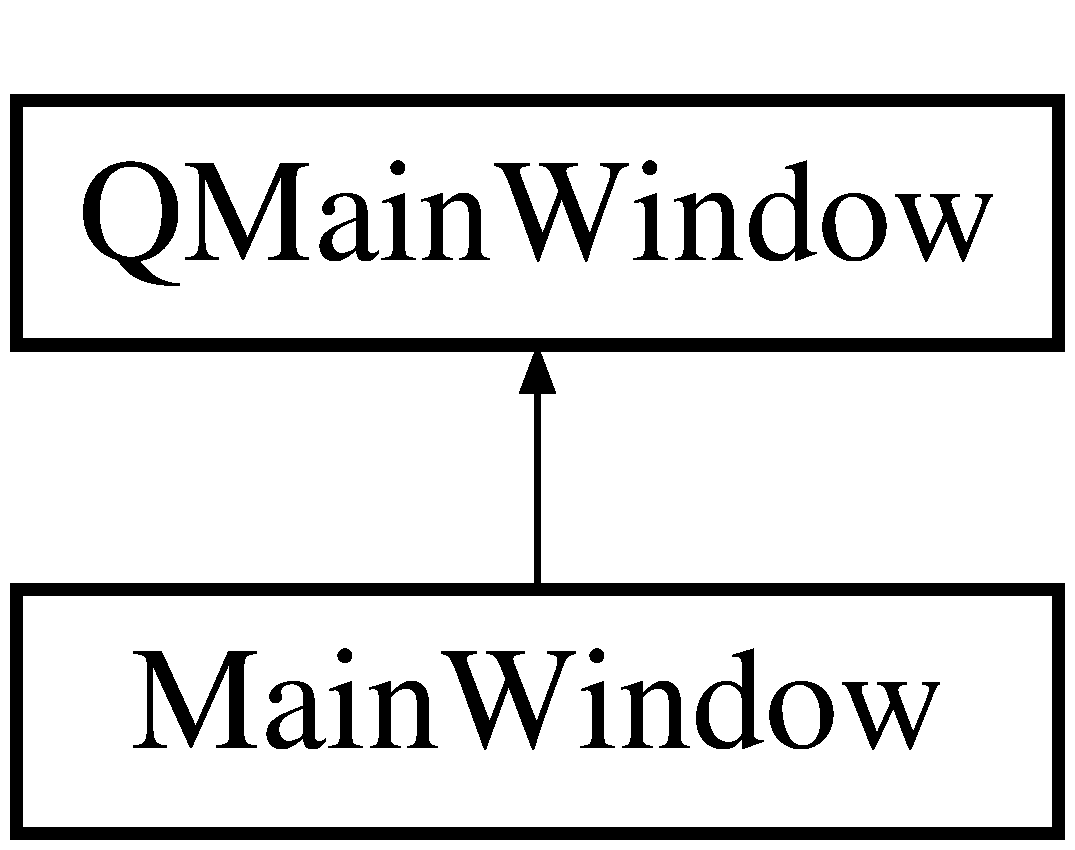
\includegraphics[height=2.000000cm]{class_main_window}
\end{center}
\end{figure}
\subsection*{Public Member Functions}
\begin{DoxyCompactItemize}
\item 
\hyperlink{class_main_window_a8b244be8b7b7db1b08de2a2acb9409db}{Main\+Window} (Q\+Widget $\ast$parent=0)
\begin{DoxyCompactList}\small\item\em The constructor. \end{DoxyCompactList}\item 
\hyperlink{class_main_window_ae98d00a93bc118200eeef9f9bba1dba7}{$\sim$\+Main\+Window} ()
\begin{DoxyCompactList}\small\item\em The Destructor. \end{DoxyCompactList}\end{DoxyCompactItemize}


\subsection{Detailed Description}
The \hyperlink{class_main_window}{Main\+Window} class. 

This class is the mother of all. It is the main window which contains all slots and widgets running the program. 

\subsection{Constructor \& Destructor Documentation}
\hypertarget{class_main_window_a8b244be8b7b7db1b08de2a2acb9409db}{}\label{class_main_window_a8b244be8b7b7db1b08de2a2acb9409db} 
\index{Main\+Window@{Main\+Window}!Main\+Window@{Main\+Window}}
\index{Main\+Window@{Main\+Window}!Main\+Window@{Main\+Window}}
\subsubsection{\texorpdfstring{Main\+Window()}{MainWindow()}}
{\footnotesize\ttfamily Main\+Window\+::\+Main\+Window (\begin{DoxyParamCaption}\item[{Q\+Widget $\ast$}]{parent = {\ttfamily 0} }\end{DoxyParamCaption})\hspace{0.3cm}{\ttfamily [explicit]}}



The constructor. 

Constructor.

It will create the main window 
\begin{DoxyParams}{Parameters}
{\em parent} & This will start the program and read all information from the files \\
\hline
\end{DoxyParams}
\hypertarget{class_main_window_ae98d00a93bc118200eeef9f9bba1dba7}{}\label{class_main_window_ae98d00a93bc118200eeef9f9bba1dba7} 
\index{Main\+Window@{Main\+Window}!````~Main\+Window@{$\sim$\+Main\+Window}}
\index{````~Main\+Window@{$\sim$\+Main\+Window}!Main\+Window@{Main\+Window}}
\subsubsection{\texorpdfstring{$\sim$\+Main\+Window()}{~MainWindow()}}
{\footnotesize\ttfamily Main\+Window\+::$\sim$\+Main\+Window (\begin{DoxyParamCaption}{ }\end{DoxyParamCaption})}



The Destructor. 

Destructor.

This will save all changes into a file and terminate the program 

The documentation for this class was generated from the following files\+:\begin{DoxyCompactItemize}
\item 
mainwindow.\+h\item 
mainwindow.\+cpp\end{DoxyCompactItemize}

\hypertarget{class_ui_1_1_main_window}{}\section{Ui\+:\+:Main\+Window Class Reference}
\label{class_ui_1_1_main_window}\index{Ui\+::\+Main\+Window@{Ui\+::\+Main\+Window}}
Inheritance diagram for Ui\+:\+:Main\+Window\+:\begin{figure}[H]
\begin{center}
\leavevmode
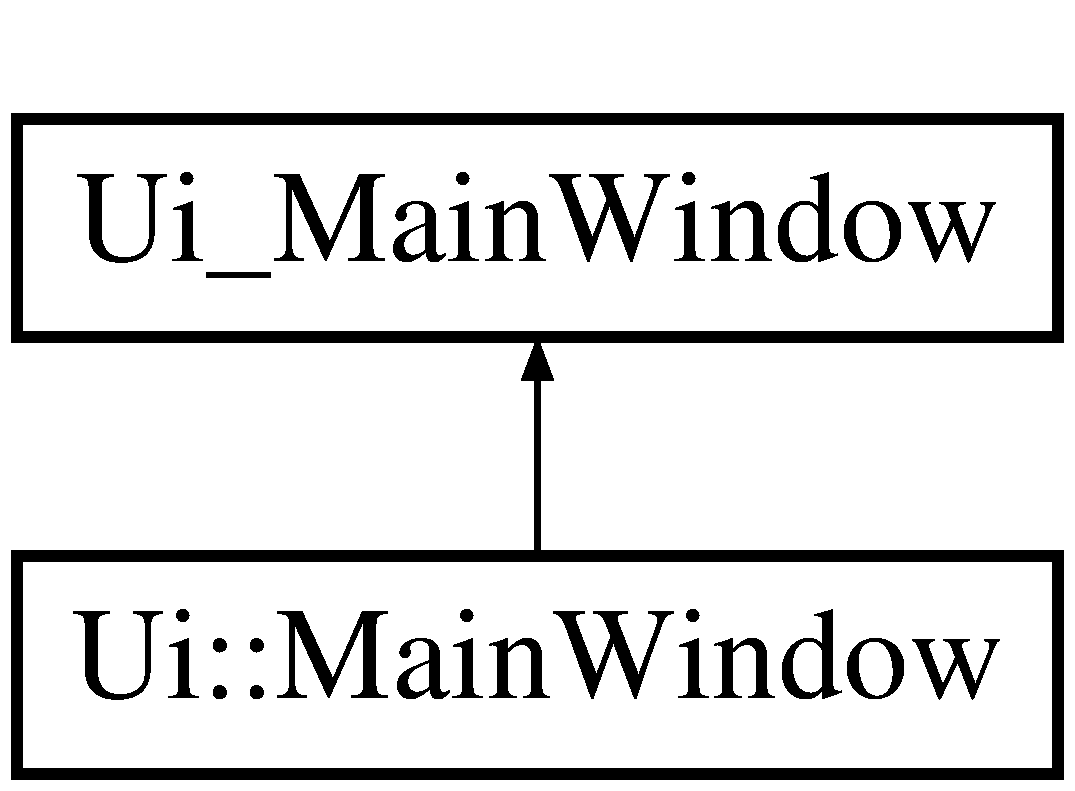
\includegraphics[height=2.000000cm]{class_ui_1_1_main_window}
\end{center}
\end{figure}
\subsection*{Additional Inherited Members}


The documentation for this class was generated from the following file\+:\begin{DoxyCompactItemize}
\item 
ui\+\_\+mainwindow.\+h\end{DoxyCompactItemize}

\hypertarget{class_ui___main_window}{}\section{Ui\+\_\+\+Main\+Window Class Reference}
\label{class_ui___main_window}\index{Ui\+\_\+\+Main\+Window@{Ui\+\_\+\+Main\+Window}}
Inheritance diagram for Ui\+\_\+\+Main\+Window\+:\begin{figure}[H]
\begin{center}
\leavevmode
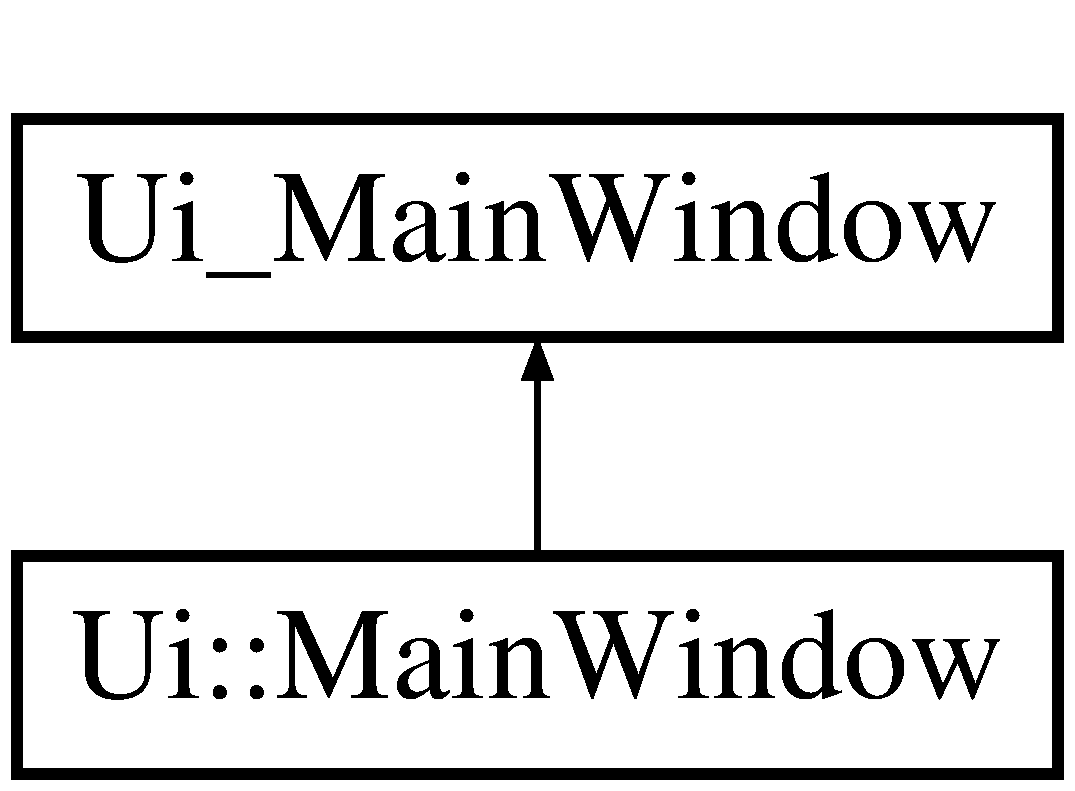
\includegraphics[height=2.000000cm]{class_ui___main_window}
\end{center}
\end{figure}
\subsection*{Public Member Functions}
\begin{DoxyCompactItemize}
\item 
\hypertarget{class_ui___main_window_acf4a0872c4c77d8f43a2ec66ed849b58}{}\label{class_ui___main_window_acf4a0872c4c77d8f43a2ec66ed849b58} 
void {\bfseries setup\+Ui} (Q\+Main\+Window $\ast$\hyperlink{class_main_window}{Main\+Window})
\item 
\hypertarget{class_ui___main_window_a097dd160c3534a204904cb374412c618}{}\label{class_ui___main_window_a097dd160c3534a204904cb374412c618} 
void {\bfseries retranslate\+Ui} (Q\+Main\+Window $\ast$\hyperlink{class_main_window}{Main\+Window})
\end{DoxyCompactItemize}
\subsection*{Public Attributes}
\begin{DoxyCompactItemize}
\item 
\hypertarget{class_ui___main_window_a84fb331a6517f83eb09fa831f2013223}{}\label{class_ui___main_window_a84fb331a6517f83eb09fa831f2013223} 
Q\+Action $\ast$ {\bfseries action\+Contact\+\_\+us}
\item 
\hypertarget{class_ui___main_window_a30075506c2116c3ed4ff25e07ae75f81}{}\label{class_ui___main_window_a30075506c2116c3ed4ff25e07ae75f81} 
Q\+Widget $\ast$ {\bfseries central\+Widget}
\item 
\hypertarget{class_ui___main_window_acd6fdc9ebacc4b25b834162380d75ce8}{}\label{class_ui___main_window_acd6fdc9ebacc4b25b834162380d75ce8} 
Q\+H\+Box\+Layout $\ast$ {\bfseries horizontal\+Layout}
\item 
\hypertarget{class_ui___main_window_a8d440a6df1de0bc57afcdda7476d8f19}{}\label{class_ui___main_window_a8d440a6df1de0bc57afcdda7476d8f19} 
Q\+Stacked\+Widget $\ast$ {\bfseries stacked\+Widget}
\item 
\hypertarget{class_ui___main_window_adfda3f701e5486d6456a704feccf7514}{}\label{class_ui___main_window_adfda3f701e5486d6456a704feccf7514} 
Q\+Widget $\ast$ {\bfseries login\+Page}
\item 
\hypertarget{class_ui___main_window_aecd96a04789fcfec3f98d80390ad8184}{}\label{class_ui___main_window_aecd96a04789fcfec3f98d80390ad8184} 
Q\+V\+Box\+Layout $\ast$ {\bfseries vertical\+Layout}
\item 
\hypertarget{class_ui___main_window_a525ed3c5fe0784ac502ee222fba4e205}{}\label{class_ui___main_window_a525ed3c5fe0784ac502ee222fba4e205} 
Q\+Grid\+Layout $\ast$ {\bfseries grid\+Layout}
\item 
\hypertarget{class_ui___main_window_a630a9bbb02ab25fd28fca1f4e61f57ec}{}\label{class_ui___main_window_a630a9bbb02ab25fd28fca1f4e61f57ec} 
Q\+Line\+Edit $\ast$ {\bfseries Edit\+Pass}
\item 
\hypertarget{class_ui___main_window_a8384329c3663ff274e926a12024aab52}{}\label{class_ui___main_window_a8384329c3663ff274e926a12024aab52} 
Q\+Spacer\+Item $\ast$ {\bfseries vertical\+Spacer}
\item 
\hypertarget{class_ui___main_window_adc1f5fdd97fb3729999c56902d0fa591}{}\label{class_ui___main_window_adc1f5fdd97fb3729999c56902d0fa591} 
Q\+Spacer\+Item $\ast$ {\bfseries vertical\+Spacer\+\_\+2}
\item 
\hypertarget{class_ui___main_window_aba69dbe102856ec3a38ec10501563264}{}\label{class_ui___main_window_aba69dbe102856ec3a38ec10501563264} 
Q\+Line\+Edit $\ast$ {\bfseries Edit\+User}
\item 
\hypertarget{class_ui___main_window_aac9fabba2c79c5c365d838576a5c1a23}{}\label{class_ui___main_window_aac9fabba2c79c5c365d838576a5c1a23} 
Q\+Push\+Button $\ast$ {\bfseries push\+Button\+\_\+exit}
\item 
\hypertarget{class_ui___main_window_a7871ea8c4b6c595d7ccd53960b344719}{}\label{class_ui___main_window_a7871ea8c4b6c595d7ccd53960b344719} 
Q\+Spacer\+Item $\ast$ {\bfseries horizontal\+Spacer}
\item 
\hypertarget{class_ui___main_window_a9a022556cf8ce3fa47e51d79cb222ab0}{}\label{class_ui___main_window_a9a022556cf8ce3fa47e51d79cb222ab0} 
Q\+Spacer\+Item $\ast$ {\bfseries horizontal\+Spacer\+\_\+2}
\item 
\hypertarget{class_ui___main_window_ad9c89133780f28e6efa2ec17ceb9cff5}{}\label{class_ui___main_window_ad9c89133780f28e6efa2ec17ceb9cff5} 
Q\+Label $\ast$ {\bfseries label}
\item 
\hypertarget{class_ui___main_window_a2e2516d755e4dd53fc905dabddf2738a}{}\label{class_ui___main_window_a2e2516d755e4dd53fc905dabddf2738a} 
Q\+Label $\ast$ {\bfseries label\+\_\+2}
\item 
\hypertarget{class_ui___main_window_ad28b2dacd95cdc7176cc0c702bd26140}{}\label{class_ui___main_window_ad28b2dacd95cdc7176cc0c702bd26140} 
Q\+Push\+Button $\ast$ {\bfseries push\+Button\+\_\+login}
\item 
\hypertarget{class_ui___main_window_aaa805963e2cb5b320863c54d734a383d}{}\label{class_ui___main_window_aaa805963e2cb5b320863c54d734a383d} 
Q\+Widget $\ast$ {\bfseries display\+Service}
\item 
\hypertarget{class_ui___main_window_a0c01bad60d9f422a1258e710635a2f65}{}\label{class_ui___main_window_a0c01bad60d9f422a1258e710635a2f65} 
Q\+V\+Box\+Layout $\ast$ {\bfseries vertical\+Layout\+\_\+2}
\item 
\hypertarget{class_ui___main_window_a6faffdc1c917d6dbcee3c2c6f2228116}{}\label{class_ui___main_window_a6faffdc1c917d6dbcee3c2c6f2228116} 
Q\+Label $\ast$ {\bfseries service\+Offers}
\item 
\hypertarget{class_ui___main_window_a4a8c3de96a17c68f56fc2f32a8b71116}{}\label{class_ui___main_window_a4a8c3de96a17c68f56fc2f32a8b71116} 
Q\+Push\+Button $\ast$ {\bfseries push\+Button\+\_\+basic}
\item 
\hypertarget{class_ui___main_window_a4c957ba501fdc47f04b020598d49db0f}{}\label{class_ui___main_window_a4c957ba501fdc47f04b020598d49db0f} 
Q\+Push\+Button $\ast$ {\bfseries push\+Button\+\_\+business}
\item 
\hypertarget{class_ui___main_window_a9f3deab9278cb121cb2a4857b12c84f6}{}\label{class_ui___main_window_a9f3deab9278cb121cb2a4857b12c84f6} 
Q\+Push\+Button $\ast$ {\bfseries push\+Button\+\_\+enterprise}
\item 
\hypertarget{class_ui___main_window_aa8715578a4a3dd71b3cf73132ac530b0}{}\label{class_ui___main_window_aa8715578a4a3dd71b3cf73132ac530b0} 
Q\+Push\+Button $\ast$ {\bfseries push\+Button\+\_\+back\+To\+Login}
\item 
\hypertarget{class_ui___main_window_aa90177c5f0bfd308f4a100e3b95c05f7}{}\label{class_ui___main_window_aa90177c5f0bfd308f4a100e3b95c05f7} 
Q\+Widget $\ast$ {\bfseries main\+Menu}
\item 
\hypertarget{class_ui___main_window_a6f40fc110b15410c00837a446d57bdbe}{}\label{class_ui___main_window_a6f40fc110b15410c00837a446d57bdbe} 
Q\+V\+Box\+Layout $\ast$ {\bfseries vertical\+Layout\+\_\+4}
\item 
\hypertarget{class_ui___main_window_a8ee86315639f324b17708efc7dbe8b19}{}\label{class_ui___main_window_a8ee86315639f324b17708efc7dbe8b19} 
Q\+Grid\+Layout $\ast$ {\bfseries grid\+Layout\+\_\+4}
\item 
\hypertarget{class_ui___main_window_a9d4bfb2fa0d87ccf9f7a311116676be6}{}\label{class_ui___main_window_a9d4bfb2fa0d87ccf9f7a311116676be6} 
Q\+Spacer\+Item $\ast$ {\bfseries vertical\+Spacer\+\_\+5}
\item 
\hypertarget{class_ui___main_window_a2e4c63737c14e5af736837df590fe004}{}\label{class_ui___main_window_a2e4c63737c14e5af736837df590fe004} 
Q\+Spacer\+Item $\ast$ {\bfseries vertical\+Spacer\+\_\+6}
\item 
\hypertarget{class_ui___main_window_a97a123cd6ffc3d9a9ebbc8c7ef871a2d}{}\label{class_ui___main_window_a97a123cd6ffc3d9a9ebbc8c7ef871a2d} 
Q\+Push\+Button $\ast$ {\bfseries push\+Button\+\_\+customers}
\item 
\hypertarget{class_ui___main_window_aca07cec23fa7d1236c8b9fe1ba9eaab1}{}\label{class_ui___main_window_aca07cec23fa7d1236c8b9fe1ba9eaab1} 
Q\+Label $\ast$ {\bfseries view\+Key\+Label}
\item 
\hypertarget{class_ui___main_window_a88478386a2833278e0565c3802fe40c3}{}\label{class_ui___main_window_a88478386a2833278e0565c3802fe40c3} 
Q\+Push\+Button $\ast$ {\bfseries push\+Button\+\_\+add\+Remove}
\item 
\hypertarget{class_ui___main_window_a4fa313108fb2b2deb5eecc911ea0ea94}{}\label{class_ui___main_window_a4fa313108fb2b2deb5eecc911ea0ea94} 
Q\+Label $\ast$ {\bfseries view\+Label}
\item 
\hypertarget{class_ui___main_window_a664e617f9dba96fb7876c39b9f28da13}{}\label{class_ui___main_window_a664e617f9dba96fb7876c39b9f28da13} 
Q\+Label $\ast$ {\bfseries add\+Label}
\item 
\hypertarget{class_ui___main_window_a8b3749e7c2b016f13823c2979f65a138}{}\label{class_ui___main_window_a8b3749e7c2b016f13823c2979f65a138} 
Q\+Push\+Button $\ast$ {\bfseries push\+Button\+\_\+key\+Customers}
\item 
\hypertarget{class_ui___main_window_a4f84e9996b7c3df489b04a7c2e57bb4d}{}\label{class_ui___main_window_a4f84e9996b7c3df489b04a7c2e57bb4d} 
Q\+Label $\ast$ {\bfseries exit\+Label}
\item 
\hypertarget{class_ui___main_window_a9410746bf57582f0dd720a5f55dedafc}{}\label{class_ui___main_window_a9410746bf57582f0dd720a5f55dedafc} 
Q\+Push\+Button $\ast$ {\bfseries push\+Button\+\_\+exit\+\_\+2}
\item 
\hypertarget{class_ui___main_window_a117e4d61a5a469a44c2016584aa04fc8}{}\label{class_ui___main_window_a117e4d61a5a469a44c2016584aa04fc8} 
Q\+Label $\ast$ {\bfseries menu\+Label}
\item 
\hypertarget{class_ui___main_window_ad332d93084584930878f1daf5f84cdbf}{}\label{class_ui___main_window_ad332d93084584930878f1daf5f84cdbf} 
Q\+Push\+Button $\ast$ {\bfseries push\+Button}
\item 
\hypertarget{class_ui___main_window_a1c16c0a684617927472e534822a63c7d}{}\label{class_ui___main_window_a1c16c0a684617927472e534822a63c7d} 
Q\+Label $\ast$ {\bfseries label\+\_\+14}
\item 
\hypertarget{class_ui___main_window_a7e0fb3338441f84ef9aa31022b757c4d}{}\label{class_ui___main_window_a7e0fb3338441f84ef9aa31022b757c4d} 
Q\+Widget $\ast$ {\bfseries View\+Customer\+\_\+2}
\item 
\hypertarget{class_ui___main_window_a38b8a4b887f3b58e2a49e7905ae6f1f0}{}\label{class_ui___main_window_a38b8a4b887f3b58e2a49e7905ae6f1f0} 
Q\+V\+Box\+Layout $\ast$ {\bfseries vertical\+Layout\+\_\+3}
\item 
\hypertarget{class_ui___main_window_a6b2a0c5f7e8ff2a87134908dd770d2d2}{}\label{class_ui___main_window_a6b2a0c5f7e8ff2a87134908dd770d2d2} 
Q\+Grid\+Layout $\ast$ {\bfseries grid\+Layout\+\_\+2}
\item 
\hypertarget{class_ui___main_window_a2295ddf43192ae3d4bcc1015743ce17c}{}\label{class_ui___main_window_a2295ddf43192ae3d4bcc1015743ce17c} 
Q\+Push\+Button $\ast$ {\bfseries push\+Button\+\_\+update\+Customer}
\item 
\hypertarget{class_ui___main_window_a77512f694ad64fe4b37d67701fbe5e16}{}\label{class_ui___main_window_a77512f694ad64fe4b37d67701fbe5e16} 
Q\+Push\+Button $\ast$ {\bfseries push\+Button\+\_\+generate\+List}
\item 
\hypertarget{class_ui___main_window_a0376fd90247280e7c7957cc70628708c}{}\label{class_ui___main_window_a0376fd90247280e7c7957cc70628708c} 
Q\+Label $\ast$ {\bfseries label\+\_\+3}
\item 
\hypertarget{class_ui___main_window_a6014826a1217c48c0c0bb1a86dc6c10a}{}\label{class_ui___main_window_a6014826a1217c48c0c0bb1a86dc6c10a} 
Q\+Push\+Button $\ast$ {\bfseries push\+Button\+\_\+view\+Customer}
\item 
\hypertarget{class_ui___main_window_a111f7e700db9586e4cd1448036c2513e}{}\label{class_ui___main_window_a111f7e700db9586e4cd1448036c2513e} 
Q\+Push\+Button $\ast$ {\bfseries push\+Button\+\_\+back}
\item 
\hypertarget{class_ui___main_window_af183bfbfb9f38bbdd60caf92b15e23dc}{}\label{class_ui___main_window_af183bfbfb9f38bbdd60caf92b15e23dc} 
Q\+Label $\ast$ {\bfseries label\+\_\+8}
\item 
\hypertarget{class_ui___main_window_aa43e1a0f9ed68685af0b2e3f09bd0302}{}\label{class_ui___main_window_aa43e1a0f9ed68685af0b2e3f09bd0302} 
Q\+List\+Widget $\ast$ {\bfseries Customer\+List}
\item 
\hypertarget{class_ui___main_window_a6596217de3ba71598a691362946589e6}{}\label{class_ui___main_window_a6596217de3ba71598a691362946589e6} 
Q\+List\+Widget $\ast$ {\bfseries Customer\+Info}
\item 
\hypertarget{class_ui___main_window_afa711e310621dd27692b6747ccfb72a0}{}\label{class_ui___main_window_afa711e310621dd27692b6747ccfb72a0} 
Q\+Widget $\ast$ {\bfseries Update\+Customer}
\item 
\hypertarget{class_ui___main_window_afcc20a3d5058037a00cdc6122f231848}{}\label{class_ui___main_window_afcc20a3d5058037a00cdc6122f231848} 
Q\+V\+Box\+Layout $\ast$ {\bfseries vertical\+Layout\+\_\+5}
\item 
\hypertarget{class_ui___main_window_af42ea7d4c2e893181caad21e28166932}{}\label{class_ui___main_window_af42ea7d4c2e893181caad21e28166932} 
Q\+Grid\+Layout $\ast$ {\bfseries grid\+Layout\+\_\+3}
\item 
\hypertarget{class_ui___main_window_ae2007c6e48638f819d3ac57be8daa4ca}{}\label{class_ui___main_window_ae2007c6e48638f819d3ac57be8daa4ca} 
Q\+Spacer\+Item $\ast$ {\bfseries horizontal\+Spacer\+\_\+3}
\item 
\hypertarget{class_ui___main_window_a8ee8ec0699ead39d0447828e51aad1e1}{}\label{class_ui___main_window_a8ee8ec0699ead39d0447828e51aad1e1} 
Q\+Line\+Edit $\ast$ {\bfseries rating}
\item 
\hypertarget{class_ui___main_window_a4fc05b11984637298795a354792c4023}{}\label{class_ui___main_window_a4fc05b11984637298795a354792c4023} 
Q\+Spacer\+Item $\ast$ {\bfseries horizontal\+Spacer\+\_\+4}
\item 
\hypertarget{class_ui___main_window_ad6bab8fb8903b8f41afea1218ee52695}{}\label{class_ui___main_window_ad6bab8fb8903b8f41afea1218ee52695} 
Q\+Label $\ast$ {\bfseries label\+\_\+5}
\item 
\hypertarget{class_ui___main_window_a298e82ba0cc2500cd61f393f493e4529}{}\label{class_ui___main_window_a298e82ba0cc2500cd61f393f493e4529} 
Q\+Spacer\+Item $\ast$ {\bfseries vertical\+Spacer\+\_\+4}
\item 
\hypertarget{class_ui___main_window_a842d5531c03b98e362e39c0cb0404ff2}{}\label{class_ui___main_window_a842d5531c03b98e362e39c0cb0404ff2} 
Q\+Push\+Button $\ast$ {\bfseries push\+Button\+\_\+update}
\item 
\hypertarget{class_ui___main_window_ac845bdf6b5b5237378a7b067808b7a31}{}\label{class_ui___main_window_ac845bdf6b5b5237378a7b067808b7a31} 
Q\+Spacer\+Item $\ast$ {\bfseries vertical\+Spacer\+\_\+3}
\item 
\hypertarget{class_ui___main_window_a78c7e10730b43c6700cd7216911ed76a}{}\label{class_ui___main_window_a78c7e10730b43c6700cd7216911ed76a} 
Q\+Label $\ast$ {\bfseries label\+\_\+4}
\item 
\hypertarget{class_ui___main_window_a6e7379663378c363756def5fd6e1bea6}{}\label{class_ui___main_window_a6e7379663378c363756def5fd6e1bea6} 
Q\+List\+Widget $\ast$ {\bfseries customer\+Info}
\item 
\hypertarget{class_ui___main_window_a4b637a76ae713711ba84a5cc51f317e1}{}\label{class_ui___main_window_a4b637a76ae713711ba84a5cc51f317e1} 
Q\+Push\+Button $\ast$ {\bfseries push\+Button\+\_\+back\+\_\+2}
\item 
\hypertarget{class_ui___main_window_a3dd88d985096d1ee2b25b201ad7fe511}{}\label{class_ui___main_window_a3dd88d985096d1ee2b25b201ad7fe511} 
Q\+Radio\+Button $\ast$ {\bfseries is\+Key\+Button}
\item 
\hypertarget{class_ui___main_window_ac4ff6e072620f9d21f155f31a5ddc71d}{}\label{class_ui___main_window_ac4ff6e072620f9d21f155f31a5ddc71d} 
Q\+Widget $\ast$ {\bfseries View\+Key\+Customer}
\item 
\hypertarget{class_ui___main_window_a7b66d5d6ab55f3977317359d09a42345}{}\label{class_ui___main_window_a7b66d5d6ab55f3977317359d09a42345} 
Q\+V\+Box\+Layout $\ast$ {\bfseries vertical\+Layout\+\_\+7}
\item 
\hypertarget{class_ui___main_window_a8731b71c513ff94baf59614807823c5d}{}\label{class_ui___main_window_a8731b71c513ff94baf59614807823c5d} 
Q\+Grid\+Layout $\ast$ {\bfseries grid\+Layout\+\_\+5}
\item 
\hypertarget{class_ui___main_window_a663f728e6244926a795c6e6892673b1d}{}\label{class_ui___main_window_a663f728e6244926a795c6e6892673b1d} 
Q\+Label $\ast$ {\bfseries label\+\_\+6}
\item 
\hypertarget{class_ui___main_window_a511cd3433fc97557a14a2bd5a0b4338c}{}\label{class_ui___main_window_a511cd3433fc97557a14a2bd5a0b4338c} 
Q\+List\+Widget $\ast$ {\bfseries Key\+Data}
\item 
\hypertarget{class_ui___main_window_a6b18450f6d4250cd35c0441dbd282a0d}{}\label{class_ui___main_window_a6b18450f6d4250cd35c0441dbd282a0d} 
Q\+Push\+Button $\ast$ {\bfseries push\+Button\+\_\+generate\+Key}
\item 
\hypertarget{class_ui___main_window_adf6745d8c1b8a0456800a7ca37924d61}{}\label{class_ui___main_window_adf6745d8c1b8a0456800a7ca37924d61} 
Q\+Push\+Button $\ast$ {\bfseries push\+Button\+\_\+view}
\item 
\hypertarget{class_ui___main_window_aa33928f3eb5593601b817641a83909ab}{}\label{class_ui___main_window_aa33928f3eb5593601b817641a83909ab} 
Q\+Push\+Button $\ast$ {\bfseries push\+Button\+\_\+back\+\_\+3}
\item 
\hypertarget{class_ui___main_window_a9f2375499484e7ca4723d6532f28499a}{}\label{class_ui___main_window_a9f2375499484e7ca4723d6532f28499a} 
Q\+List\+Widget $\ast$ {\bfseries Key\+List}
\item 
\hypertarget{class_ui___main_window_a609b04cadea67e89d037fd377074cf3d}{}\label{class_ui___main_window_a609b04cadea67e89d037fd377074cf3d} 
Q\+Widget $\ast$ {\bfseries Add\+Remove}
\item 
\hypertarget{class_ui___main_window_a93c190b085c63a667c535ba0bbcfec7c}{}\label{class_ui___main_window_a93c190b085c63a667c535ba0bbcfec7c} 
Q\+V\+Box\+Layout $\ast$ {\bfseries vertical\+Layout\+\_\+6}
\item 
\hypertarget{class_ui___main_window_ad113cf7b76aaf178473555bdf64ff035}{}\label{class_ui___main_window_ad113cf7b76aaf178473555bdf64ff035} 
Q\+Grid\+Layout $\ast$ {\bfseries grid\+Layout\+\_\+6}
\item 
\hypertarget{class_ui___main_window_afaed76f493357f7aaa5ee48f6cf7fe50}{}\label{class_ui___main_window_afaed76f493357f7aaa5ee48f6cf7fe50} 
Q\+Line\+Edit $\ast$ {\bfseries line\+Edit\+\_\+address\+\_\+2}
\item 
\hypertarget{class_ui___main_window_aa2621565827195e88436fb54220bb48d}{}\label{class_ui___main_window_aa2621565827195e88436fb54220bb48d} 
Q\+Label $\ast$ {\bfseries label\+\_\+12}
\item 
\hypertarget{class_ui___main_window_a71605bcf74c938f64207451850fc69b1}{}\label{class_ui___main_window_a71605bcf74c938f64207451850fc69b1} 
Q\+Spacer\+Item $\ast$ {\bfseries horizontal\+Spacer\+\_\+5}
\item 
\hypertarget{class_ui___main_window_a5c942fe3a559acafdddc79365ddf5558}{}\label{class_ui___main_window_a5c942fe3a559acafdddc79365ddf5558} 
Q\+Line\+Edit $\ast$ {\bfseries line\+Edit\+\_\+address\+\_\+1}
\item 
\hypertarget{class_ui___main_window_a7144de5a0bec057362d4dd43e30844af}{}\label{class_ui___main_window_a7144de5a0bec057362d4dd43e30844af} 
Q\+Line\+Edit $\ast$ {\bfseries line\+Edit\+\_\+customer\+Name}
\item 
\hypertarget{class_ui___main_window_a0e90c7e9ad77386881e0b264ddb9dd22}{}\label{class_ui___main_window_a0e90c7e9ad77386881e0b264ddb9dd22} 
Q\+Label $\ast$ {\bfseries label\+\_\+9}
\item 
\hypertarget{class_ui___main_window_ad288a5d40e2775444e0feb40e1b99289}{}\label{class_ui___main_window_ad288a5d40e2775444e0feb40e1b99289} 
Q\+Push\+Button $\ast$ {\bfseries push\+Button\+\_\+back\+\_\+4}
\item 
\hypertarget{class_ui___main_window_ac554123dda4b7f53eaf995feecef2aa1}{}\label{class_ui___main_window_ac554123dda4b7f53eaf995feecef2aa1} 
Q\+Spacer\+Item $\ast$ {\bfseries vertical\+Spacer\+\_\+8}
\item 
\hypertarget{class_ui___main_window_ae6aa3f2ea7a5ff106015aa6ef9f24529}{}\label{class_ui___main_window_ae6aa3f2ea7a5ff106015aa6ef9f24529} 
Q\+Spacer\+Item $\ast$ {\bfseries vertical\+Spacer\+\_\+7}
\item 
\hypertarget{class_ui___main_window_a13936e6f18b1c90402b3c7a3c92b6cdb}{}\label{class_ui___main_window_a13936e6f18b1c90402b3c7a3c92b6cdb} 
Q\+Label $\ast$ {\bfseries label\+\_\+7}
\item 
\hypertarget{class_ui___main_window_ac1cbc41e9dbaeb3d0bdc2189d8e9ee1d}{}\label{class_ui___main_window_ac1cbc41e9dbaeb3d0bdc2189d8e9ee1d} 
Q\+Label $\ast$ {\bfseries label\+\_\+13}
\item 
\hypertarget{class_ui___main_window_a17edf36d941b89705725785c726872b5}{}\label{class_ui___main_window_a17edf36d941b89705725785c726872b5} 
Q\+Push\+Button $\ast$ {\bfseries push\+Button\+\_\+remove}
\item 
\hypertarget{class_ui___main_window_a58850298c543f4d86b5a45f35f1b886a}{}\label{class_ui___main_window_a58850298c543f4d86b5a45f35f1b886a} 
Q\+Push\+Button $\ast$ {\bfseries push\+Button\+\_\+add}
\item 
\hypertarget{class_ui___main_window_a3202b80ffde7629da626c1e0994f63f5}{}\label{class_ui___main_window_a3202b80ffde7629da626c1e0994f63f5} 
Q\+Spacer\+Item $\ast$ {\bfseries horizontal\+Spacer\+\_\+6}
\item 
\hypertarget{class_ui___main_window_ab0fe5a3bb0fbeb730223449fcd69ed27}{}\label{class_ui___main_window_ab0fe5a3bb0fbeb730223449fcd69ed27} 
Q\+Line\+Edit $\ast$ {\bfseries line\+Edit\+\_\+password}
\item 
\hypertarget{class_ui___main_window_ab6ac4329a89041f557332f6569d94493}{}\label{class_ui___main_window_ab6ac4329a89041f557332f6569d94493} 
Q\+Label $\ast$ {\bfseries label\+\_\+16}
\item 
\hypertarget{class_ui___main_window_aef083f5fb8e2be926b194c85f82abe35}{}\label{class_ui___main_window_aef083f5fb8e2be926b194c85f82abe35} 
Q\+Line\+Edit $\ast$ {\bfseries line\+Edit\+\_\+rating}
\item 
\hypertarget{class_ui___main_window_a4f12a71b4a2fb6f85df2300d83b5ed3e}{}\label{class_ui___main_window_a4f12a71b4a2fb6f85df2300d83b5ed3e} 
Q\+Label $\ast$ {\bfseries label\+\_\+11}
\item 
\hypertarget{class_ui___main_window_a61269a10bc342763a5a51a93a235944d}{}\label{class_ui___main_window_a61269a10bc342763a5a51a93a235944d} 
Q\+Radio\+Button $\ast$ {\bfseries radio\+Button}
\item 
\hypertarget{class_ui___main_window_a9dc4dba26b83e0c94aa566e1c564420b}{}\label{class_ui___main_window_a9dc4dba26b83e0c94aa566e1c564420b} 
Q\+Label $\ast$ {\bfseries label\+\_\+10}
\item 
\hypertarget{class_ui___main_window_a2be1c24ec9adfca18e1dcc951931457f}{}\label{class_ui___main_window_a2be1c24ec9adfca18e1dcc951931457f} 
Q\+Menu\+Bar $\ast$ {\bfseries menu\+Bar}
\item 
\hypertarget{class_ui___main_window_a0959e3924382c51bb75157b6fc85c6e3}{}\label{class_ui___main_window_a0959e3924382c51bb75157b6fc85c6e3} 
Q\+Menu $\ast$ {\bfseries menu\+Contact\+\_\+us}
\item 
\hypertarget{class_ui___main_window_a5172877001c8c7b4e0f6de50421867d1}{}\label{class_ui___main_window_a5172877001c8c7b4e0f6de50421867d1} 
Q\+Tool\+Bar $\ast$ {\bfseries main\+Tool\+Bar}
\item 
\hypertarget{class_ui___main_window_a50fa481337604bcc8bf68de18ab16ecd}{}\label{class_ui___main_window_a50fa481337604bcc8bf68de18ab16ecd} 
Q\+Status\+Bar $\ast$ {\bfseries status\+Bar}
\end{DoxyCompactItemize}


The documentation for this class was generated from the following file\+:\begin{DoxyCompactItemize}
\item 
ui\+\_\+mainwindow.\+h\end{DoxyCompactItemize}

\hypertarget{structuser}{}\section{user Struct Reference}
\label{structuser}\index{user@{user}}


The user struct.  




{\ttfamily \#include $<$readrite.\+h$>$}

\subsection*{Public Attributes}
\begin{DoxyCompactItemize}
\item 
\hypertarget{structuser_ad044cc7054ee3116809f97698017eb49}{}\label{structuser_ad044cc7054ee3116809f97698017eb49} 
Q\+String {\bfseries name}
\item 
\hypertarget{structuser_a2b1a33adf680f13f15e5071f73e0279f}{}\label{structuser_a2b1a33adf680f13f15e5071f73e0279f} 
Q\+String {\bfseries password}
\item 
\hypertarget{structuser_a2e40bf8fed819f9b7d98a38f2227f524}{}\label{structuser_a2e40bf8fed819f9b7d98a38f2227f524} 
Q\+String {\bfseries address1}
\item 
\hypertarget{structuser_a2d0ec864894b448db9360fba7052672a}{}\label{structuser_a2d0ec864894b448db9360fba7052672a} 
Q\+String {\bfseries address2}
\item 
\hypertarget{structuser_a12e18612bc94f5c63b27c5e432946765}{}\label{structuser_a12e18612bc94f5c63b27c5e432946765} 
Q\+String {\bfseries intrest\+Level}
\item 
\hypertarget{structuser_a1230fdce012d16fd66ebde09e760b87d}{}\label{structuser_a1230fdce012d16fd66ebde09e760b87d} 
bool {\bfseries is\+Key}
\end{DoxyCompactItemize}


\subsection{Detailed Description}
The user struct. 

This is the user struct to hold the respective fields related to a customer. 

The documentation for this struct was generated from the following file\+:\begin{DoxyCompactItemize}
\item 
readrite.\+h\end{DoxyCompactItemize}

\hypertarget{classvector}{}\section{vector$<$ Type $>$ Class Template Reference}
\label{classvector}\index{vector$<$ Type $>$@{vector$<$ Type $>$}}


Template Vector class.  




{\ttfamily \#include $<$vector.\+h$>$}

\subsection*{Public Types}
\begin{DoxyCompactItemize}
\item 
\hypertarget{classvector_a0353117bdb832ae6616b6a068f8258da}{}\label{classvector_a0353117bdb832ae6616b6a068f8258da} 
typedef Type $\ast$ {\bfseries iterator}
\item 
\hypertarget{classvector_a574b95e8b5195d74bc6d1d9c530cf8b0}{}\label{classvector_a574b95e8b5195d74bc6d1d9c530cf8b0} 
typedef Type {\bfseries const\+\_\+iterator}
\end{DoxyCompactItemize}
\subsection*{Public Member Functions}
\begin{DoxyCompactItemize}
\item 
\hyperlink{classvector_ab8d8ebaa9b91a05bb7a94371cb84c042}{vector} ()
\begin{DoxyCompactList}\small\item\em \hyperlink{classvector_ab8d8ebaa9b91a05bb7a94371cb84c042}{vector()} -\/ Constructor \end{DoxyCompactList}\item 
\hyperlink{classvector_a98cdf37dc536057976131f5f9bb8e402}{vector} (int s)
\begin{DoxyCompactList}\small\item\em \hyperlink{classvector_ab8d8ebaa9b91a05bb7a94371cb84c042}{vector()} -\/ Constructor alternate \end{DoxyCompactList}\item 
\hyperlink{classvector_a09bcb733130a4b75eab388d79a6ad1c6}{vector} (const \hyperlink{classvector}{vector} \&src)
\begin{DoxyCompactList}\small\item\em \hyperlink{classvector_ab8d8ebaa9b91a05bb7a94371cb84c042}{vector()} -\/ Copy Constructor \end{DoxyCompactList}\item 
\hyperlink{classvector}{vector} \& \hyperlink{classvector_a4de09f8f1844cead9daef18122e3cdf6}{operator=} (const \hyperlink{classvector}{vector} \&src)
\begin{DoxyCompactList}\small\item\em \hyperlink{classvector_ab8d8ebaa9b91a05bb7a94371cb84c042}{vector()} -\/ Assignment operator \end{DoxyCompactList}\item 
\hypertarget{classvector_afbb927ea4d353b71b4b5cd13fa67d598}{}\label{classvector_afbb927ea4d353b71b4b5cd13fa67d598} 
{\bfseries vector} (\hyperlink{classvector}{vector}$<$ Type $>$ \&)
\item 
\hyperlink{classvector}{vector} \& \hyperlink{classvector_acbbf4dfffea32b7145d7bb24dd3a0df2}{operator=} (\hyperlink{classvector}{vector} \&)
\begin{DoxyCompactList}\small\item\em \hyperlink{classvector_ab8d8ebaa9b91a05bb7a94371cb84c042}{vector()} -\/ Assignment operator \end{DoxyCompactList}\item 
\hyperlink{classvector_af6ca21dc63ee5974d306c5c4ad104294}{$\sim$vector} ()
\begin{DoxyCompactList}\small\item\em \hyperlink{classvector_ab8d8ebaa9b91a05bb7a94371cb84c042}{vector()} -\/ Destructor \end{DoxyCompactList}\item 
Type \& \hyperlink{classvector_ae7389576636ca0117a731ed2626ac747}{operator\mbox{[}$\,$\mbox{]}} (int n)
\begin{DoxyCompactList}\small\item\em \hyperlink{classvector_ab8d8ebaa9b91a05bb7a94371cb84c042}{vector()} -\/ operator\mbox{[}\mbox{]} \end{DoxyCompactList}\item 
const Type \& \hyperlink{classvector_ae7ec6942e0a373dc03c99796ce3555eb}{operator\mbox{[}$\,$\mbox{]}} (int n) const
\begin{DoxyCompactList}\small\item\em \hyperlink{classvector_ab8d8ebaa9b91a05bb7a94371cb84c042}{vector()} -\/ const operator\mbox{[}\mbox{]} \end{DoxyCompactList}\item 
int \hyperlink{classvector_a0c650d6f1411947dc6a407c4adde5109}{get\+Size} () const
\begin{DoxyCompactList}\small\item\em \hyperlink{classvector_ab8d8ebaa9b91a05bb7a94371cb84c042}{vector()} -\/ get\+Size \end{DoxyCompactList}\item 
int \hyperlink{classvector_a9f64c11bb3348e2d1c5c4f41ae15780f}{get\+Space} () const
\begin{DoxyCompactList}\small\item\em \hyperlink{classvector_ab8d8ebaa9b91a05bb7a94371cb84c042}{vector()} -\/ get\+Space \end{DoxyCompactList}\item 
void \hyperlink{classvector_acb1ede35cda295c9e1729ca981d39e09}{reserve} (int new\+Alloc)
\begin{DoxyCompactList}\small\item\em \hyperlink{classvector_ab8d8ebaa9b91a05bb7a94371cb84c042}{vector()} -\/ reserve \end{DoxyCompactList}\item 
void \hyperlink{classvector_a3e51ccc704255ec4acfed8e3d5c7be7f}{resize} (int new\+Size)
\begin{DoxyCompactList}\small\item\em \hyperlink{classvector_ab8d8ebaa9b91a05bb7a94371cb84c042}{vector()} -\/ resize \end{DoxyCompactList}\item 
void \hyperlink{classvector_aa09467ef9ad6c97aa952cdbff9085400}{push\+\_\+back} (Type new\+Elem)
\begin{DoxyCompactList}\small\item\em \hyperlink{classvector_ab8d8ebaa9b91a05bb7a94371cb84c042}{vector()} -\/ push Back \end{DoxyCompactList}\item 
void \hyperlink{classvector_a427b0c894a09dd7d57f46b341fad95a5}{del\+Elem} (int del\+Elem)
\begin{DoxyCompactList}\small\item\em \hyperlink{classvector_ab8d8ebaa9b91a05bb7a94371cb84c042}{vector()} -\/ delete element \end{DoxyCompactList}\item 
iterator \hyperlink{classvector_a1a2e2bce9c55489fc3c65ea6956a8c8d}{begin} ()
\begin{DoxyCompactList}\small\item\em iterator -\/ begin \end{DoxyCompactList}\item 
const\+\_\+iterator \hyperlink{classvector_a4e799b72c6f027170e5ae7145746abf1}{begin} () const
\begin{DoxyCompactList}\small\item\em iterator -\/ const begin \end{DoxyCompactList}\item 
iterator \hyperlink{classvector_a37658994f03de8e7e2122a24877169f5}{end} ()
\begin{DoxyCompactList}\small\item\em iterator -\/ end \end{DoxyCompactList}\item 
const\+\_\+iterator \hyperlink{classvector_ab07ef3f43e79f9e9e5080ccaaab6cfd2}{end} () const
\begin{DoxyCompactList}\small\item\em iterator -\/ const end \end{DoxyCompactList}\item 
iterator \hyperlink{classvector_ae416d913721ccee87128230e0ff9a5fa}{insert} (iterator location, const Type \&val)
\begin{DoxyCompactList}\small\item\em iterator -\/ insert \end{DoxyCompactList}\item 
iterator \hyperlink{classvector_afd19d0871c27f1e2d216749f542cd0ca}{find} (Type val)
\begin{DoxyCompactList}\small\item\em iterator -\/ find \end{DoxyCompactList}\item 
void \hyperlink{classvector_a07b7c89f4914f1558409e81ca0fe4e72}{sort} ()
\begin{DoxyCompactList}\small\item\em iterator -\/ sort \end{DoxyCompactList}\end{DoxyCompactItemize}


\subsection{Detailed Description}
\subsubsection*{template$<$class Type$>$\newline
class vector$<$ Type $>$}

Template Vector class. 

This templated vector class will allow us to store any type of data into the vector and use it as a container to hold all customers 

\subsection{Constructor \& Destructor Documentation}
\hypertarget{classvector_ab8d8ebaa9b91a05bb7a94371cb84c042}{}\label{classvector_ab8d8ebaa9b91a05bb7a94371cb84c042} 
\index{vector@{vector}!vector@{vector}}
\index{vector@{vector}!vector@{vector}}
\subsubsection{\texorpdfstring{vector()}{vector()}\hspace{0.1cm}{\footnotesize\ttfamily [1/3]}}
{\footnotesize\ttfamily template$<$class Type$>$ \\
\hyperlink{classvector}{vector}$<$ Type $>$\+::\hyperlink{classvector}{vector} (\begin{DoxyParamCaption}{ }\end{DoxyParamCaption})\hspace{0.3cm}{\ttfamily [inline]}}



\hyperlink{classvector_ab8d8ebaa9b91a05bb7a94371cb84c042}{vector()} -\/ Constructor 

This will initialize the constructor \hypertarget{classvector_a98cdf37dc536057976131f5f9bb8e402}{}\label{classvector_a98cdf37dc536057976131f5f9bb8e402} 
\index{vector@{vector}!vector@{vector}}
\index{vector@{vector}!vector@{vector}}
\subsubsection{\texorpdfstring{vector()}{vector()}\hspace{0.1cm}{\footnotesize\ttfamily [2/3]}}
{\footnotesize\ttfamily template$<$class Type$>$ \\
\hyperlink{classvector}{vector}$<$ Type $>$\+::\hyperlink{classvector}{vector} (\begin{DoxyParamCaption}\item[{int}]{s }\end{DoxyParamCaption})\hspace{0.3cm}{\ttfamily [inline]}, {\ttfamily [explicit]}}



\hyperlink{classvector_ab8d8ebaa9b91a05bb7a94371cb84c042}{vector()} -\/ Constructor alternate 

This will initialize the constructor \hypertarget{classvector_a09bcb733130a4b75eab388d79a6ad1c6}{}\label{classvector_a09bcb733130a4b75eab388d79a6ad1c6} 
\index{vector@{vector}!vector@{vector}}
\index{vector@{vector}!vector@{vector}}
\subsubsection{\texorpdfstring{vector()}{vector()}\hspace{0.1cm}{\footnotesize\ttfamily [3/3]}}
{\footnotesize\ttfamily template$<$class Type$>$ \\
\hyperlink{classvector}{vector}$<$ Type $>$\+::\hyperlink{classvector}{vector} (\begin{DoxyParamCaption}\item[{const \hyperlink{classvector}{vector}$<$ Type $>$ \&}]{src }\end{DoxyParamCaption})\hspace{0.3cm}{\ttfamily [inline]}}



\hyperlink{classvector_ab8d8ebaa9b91a05bb7a94371cb84c042}{vector()} -\/ Copy Constructor 

This will copy another vector into our vector \hypertarget{classvector_af6ca21dc63ee5974d306c5c4ad104294}{}\label{classvector_af6ca21dc63ee5974d306c5c4ad104294} 
\index{vector@{vector}!````~vector@{$\sim$vector}}
\index{````~vector@{$\sim$vector}!vector@{vector}}
\subsubsection{\texorpdfstring{$\sim$vector()}{~vector()}}
{\footnotesize\ttfamily template$<$class Type$>$ \\
\hyperlink{classvector}{vector}$<$ Type $>$\+::$\sim$\hyperlink{classvector}{vector} (\begin{DoxyParamCaption}{ }\end{DoxyParamCaption})\hspace{0.3cm}{\ttfamily [inline]}}



\hyperlink{classvector_ab8d8ebaa9b91a05bb7a94371cb84c042}{vector()} -\/ Destructor 

This will destroy all elements from the vector 

\subsection{Member Function Documentation}
\hypertarget{classvector_a1a2e2bce9c55489fc3c65ea6956a8c8d}{}\label{classvector_a1a2e2bce9c55489fc3c65ea6956a8c8d} 
\index{vector@{vector}!begin@{begin}}
\index{begin@{begin}!vector@{vector}}
\subsubsection{\texorpdfstring{begin()}{begin()}\hspace{0.1cm}{\footnotesize\ttfamily [1/2]}}
{\footnotesize\ttfamily template$<$class Type$>$ \\
iterator \hyperlink{classvector}{vector}$<$ Type $>$\+::begin (\begin{DoxyParamCaption}{ }\end{DoxyParamCaption})\hspace{0.3cm}{\ttfamily [inline]}}



iterator -\/ begin 

This will return the address of the first element in the vector \hypertarget{classvector_a4e799b72c6f027170e5ae7145746abf1}{}\label{classvector_a4e799b72c6f027170e5ae7145746abf1} 
\index{vector@{vector}!begin@{begin}}
\index{begin@{begin}!vector@{vector}}
\subsubsection{\texorpdfstring{begin()}{begin()}\hspace{0.1cm}{\footnotesize\ttfamily [2/2]}}
{\footnotesize\ttfamily template$<$class Type$>$ \\
const\+\_\+iterator \hyperlink{classvector}{vector}$<$ Type $>$\+::begin (\begin{DoxyParamCaption}{ }\end{DoxyParamCaption}) const\hspace{0.3cm}{\ttfamily [inline]}}



iterator -\/ const begin 

This will return the address of the first element in the vector \hypertarget{classvector_a427b0c894a09dd7d57f46b341fad95a5}{}\label{classvector_a427b0c894a09dd7d57f46b341fad95a5} 
\index{vector@{vector}!del\+Elem@{del\+Elem}}
\index{del\+Elem@{del\+Elem}!vector@{vector}}
\subsubsection{\texorpdfstring{del\+Elem()}{delElem()}}
{\footnotesize\ttfamily template$<$class Type$>$ \\
void \hyperlink{classvector}{vector}$<$ Type $>$\+::del\+Elem (\begin{DoxyParamCaption}\item[{int}]{del\+Elem }\end{DoxyParamCaption})\hspace{0.3cm}{\ttfamily [inline]}}



\hyperlink{classvector_ab8d8ebaa9b91a05bb7a94371cb84c042}{vector()} -\/ delete element 

This will remove an element from the vector New array with one less element

Is incremented after element deletion to prevent skipping an index

Copies elements from the old array unless index matches del\+Elem

Increments f if index matches del\+Elem \hypertarget{classvector_a37658994f03de8e7e2122a24877169f5}{}\label{classvector_a37658994f03de8e7e2122a24877169f5} 
\index{vector@{vector}!end@{end}}
\index{end@{end}!vector@{vector}}
\subsubsection{\texorpdfstring{end()}{end()}\hspace{0.1cm}{\footnotesize\ttfamily [1/2]}}
{\footnotesize\ttfamily template$<$class Type$>$ \\
iterator \hyperlink{classvector}{vector}$<$ Type $>$\+::end (\begin{DoxyParamCaption}{ }\end{DoxyParamCaption})\hspace{0.3cm}{\ttfamily [inline]}}



iterator -\/ end 

This will return the address of the last element in the vector \hypertarget{classvector_ab07ef3f43e79f9e9e5080ccaaab6cfd2}{}\label{classvector_ab07ef3f43e79f9e9e5080ccaaab6cfd2} 
\index{vector@{vector}!end@{end}}
\index{end@{end}!vector@{vector}}
\subsubsection{\texorpdfstring{end()}{end()}\hspace{0.1cm}{\footnotesize\ttfamily [2/2]}}
{\footnotesize\ttfamily template$<$class Type$>$ \\
const\+\_\+iterator \hyperlink{classvector}{vector}$<$ Type $>$\+::end (\begin{DoxyParamCaption}{ }\end{DoxyParamCaption}) const\hspace{0.3cm}{\ttfamily [inline]}}



iterator -\/ const end 

This will return the address of the last element in the vector \hypertarget{classvector_afd19d0871c27f1e2d216749f542cd0ca}{}\label{classvector_afd19d0871c27f1e2d216749f542cd0ca} 
\index{vector@{vector}!find@{find}}
\index{find@{find}!vector@{vector}}
\subsubsection{\texorpdfstring{find()}{find()}}
{\footnotesize\ttfamily template$<$class Type$>$ \\
iterator \hyperlink{classvector}{vector}$<$ Type $>$\+::find (\begin{DoxyParamCaption}\item[{Type}]{val }\end{DoxyParamCaption})\hspace{0.3cm}{\ttfamily [inline]}}



iterator -\/ find 

This will find the specified value in the vector and return its address \hypertarget{classvector_a0c650d6f1411947dc6a407c4adde5109}{}\label{classvector_a0c650d6f1411947dc6a407c4adde5109} 
\index{vector@{vector}!get\+Size@{get\+Size}}
\index{get\+Size@{get\+Size}!vector@{vector}}
\subsubsection{\texorpdfstring{get\+Size()}{getSize()}}
{\footnotesize\ttfamily template$<$class Type$>$ \\
int \hyperlink{classvector}{vector}$<$ Type $>$\+::get\+Size (\begin{DoxyParamCaption}{ }\end{DoxyParamCaption}) const\hspace{0.3cm}{\ttfamily [inline]}}



\hyperlink{classvector_ab8d8ebaa9b91a05bb7a94371cb84c042}{vector()} -\/ get\+Size 

This will return the size of vector \hypertarget{classvector_a9f64c11bb3348e2d1c5c4f41ae15780f}{}\label{classvector_a9f64c11bb3348e2d1c5c4f41ae15780f} 
\index{vector@{vector}!get\+Space@{get\+Space}}
\index{get\+Space@{get\+Space}!vector@{vector}}
\subsubsection{\texorpdfstring{get\+Space()}{getSpace()}}
{\footnotesize\ttfamily template$<$class Type$>$ \\
int \hyperlink{classvector}{vector}$<$ Type $>$\+::get\+Space (\begin{DoxyParamCaption}{ }\end{DoxyParamCaption}) const\hspace{0.3cm}{\ttfamily [inline]}}



\hyperlink{classvector_ab8d8ebaa9b91a05bb7a94371cb84c042}{vector()} -\/ get\+Space 

This will return the space of the vector \hypertarget{classvector_ae416d913721ccee87128230e0ff9a5fa}{}\label{classvector_ae416d913721ccee87128230e0ff9a5fa} 
\index{vector@{vector}!insert@{insert}}
\index{insert@{insert}!vector@{vector}}
\subsubsection{\texorpdfstring{insert()}{insert()}}
{\footnotesize\ttfamily template$<$class Type$>$ \\
iterator \hyperlink{classvector}{vector}$<$ Type $>$\+::insert (\begin{DoxyParamCaption}\item[{iterator}]{location,  }\item[{const Type \&}]{val }\end{DoxyParamCaption})\hspace{0.3cm}{\ttfamily [inline]}}



iterator -\/ insert 

This will insert an elemtn at the \char`\"{}location\char`\"{} index \hypertarget{classvector_a4de09f8f1844cead9daef18122e3cdf6}{}\label{classvector_a4de09f8f1844cead9daef18122e3cdf6} 
\index{vector@{vector}!operator=@{operator=}}
\index{operator=@{operator=}!vector@{vector}}
\subsubsection{\texorpdfstring{operator=()}{operator=()}\hspace{0.1cm}{\footnotesize\ttfamily [1/2]}}
{\footnotesize\ttfamily template$<$class Type$>$ \\
\hyperlink{classvector}{vector}\& \hyperlink{classvector}{vector}$<$ Type $>$\+::operator= (\begin{DoxyParamCaption}\item[{const \hyperlink{classvector}{vector}$<$ Type $>$ \&}]{src }\end{DoxyParamCaption})\hspace{0.3cm}{\ttfamily [inline]}}



\hyperlink{classvector_ab8d8ebaa9b91a05bb7a94371cb84c042}{vector()} -\/ Assignment operator 

This will allow to user the assignment opeartor \hypertarget{classvector_acbbf4dfffea32b7145d7bb24dd3a0df2}{}\label{classvector_acbbf4dfffea32b7145d7bb24dd3a0df2} 
\index{vector@{vector}!operator=@{operator=}}
\index{operator=@{operator=}!vector@{vector}}
\subsubsection{\texorpdfstring{operator=()}{operator=()}\hspace{0.1cm}{\footnotesize\ttfamily [2/2]}}
{\footnotesize\ttfamily template$<$class Type$>$ \\
\hyperlink{classvector}{vector}\& \hyperlink{classvector}{vector}$<$ Type $>$\+::operator= (\begin{DoxyParamCaption}\item[{\hyperlink{classvector}{vector}$<$ Type $>$ \&}]{ }\end{DoxyParamCaption})}



\hyperlink{classvector_ab8d8ebaa9b91a05bb7a94371cb84c042}{vector()} -\/ Assignment operator 

This will allow to user the assignment opeartor \hypertarget{classvector_ae7389576636ca0117a731ed2626ac747}{}\label{classvector_ae7389576636ca0117a731ed2626ac747} 
\index{vector@{vector}!operator\mbox{[}\mbox{]}@{operator[]}}
\index{operator\mbox{[}\mbox{]}@{operator[]}!vector@{vector}}
\subsubsection{\texorpdfstring{operator[]()}{operator[]()}\hspace{0.1cm}{\footnotesize\ttfamily [1/2]}}
{\footnotesize\ttfamily template$<$class Type$>$ \\
Type\& \hyperlink{classvector}{vector}$<$ Type $>$\+::operator\mbox{[}$\,$\mbox{]} (\begin{DoxyParamCaption}\item[{int}]{n }\end{DoxyParamCaption})\hspace{0.3cm}{\ttfamily [inline]}}



\hyperlink{classvector_ab8d8ebaa9b91a05bb7a94371cb84c042}{vector()} -\/ operator\mbox{[}\mbox{]} 

This will return the element n in the vector \hypertarget{classvector_ae7ec6942e0a373dc03c99796ce3555eb}{}\label{classvector_ae7ec6942e0a373dc03c99796ce3555eb} 
\index{vector@{vector}!operator\mbox{[}\mbox{]}@{operator[]}}
\index{operator\mbox{[}\mbox{]}@{operator[]}!vector@{vector}}
\subsubsection{\texorpdfstring{operator[]()}{operator[]()}\hspace{0.1cm}{\footnotesize\ttfamily [2/2]}}
{\footnotesize\ttfamily template$<$class Type$>$ \\
const Type\& \hyperlink{classvector}{vector}$<$ Type $>$\+::operator\mbox{[}$\,$\mbox{]} (\begin{DoxyParamCaption}\item[{int}]{n }\end{DoxyParamCaption}) const\hspace{0.3cm}{\ttfamily [inline]}}



\hyperlink{classvector_ab8d8ebaa9b91a05bb7a94371cb84c042}{vector()} -\/ const operator\mbox{[}\mbox{]} 

This will return the element n in the vector \hypertarget{classvector_aa09467ef9ad6c97aa952cdbff9085400}{}\label{classvector_aa09467ef9ad6c97aa952cdbff9085400} 
\index{vector@{vector}!push\+\_\+back@{push\+\_\+back}}
\index{push\+\_\+back@{push\+\_\+back}!vector@{vector}}
\subsubsection{\texorpdfstring{push\+\_\+back()}{push\_back()}}
{\footnotesize\ttfamily template$<$class Type$>$ \\
void \hyperlink{classvector}{vector}$<$ Type $>$\+::push\+\_\+back (\begin{DoxyParamCaption}\item[{Type}]{new\+Elem }\end{DoxyParamCaption})\hspace{0.3cm}{\ttfamily [inline]}}



\hyperlink{classvector_ab8d8ebaa9b91a05bb7a94371cb84c042}{vector()} -\/ push Back 

This will push new elemnts into the vector at the end \hypertarget{classvector_acb1ede35cda295c9e1729ca981d39e09}{}\label{classvector_acb1ede35cda295c9e1729ca981d39e09} 
\index{vector@{vector}!reserve@{reserve}}
\index{reserve@{reserve}!vector@{vector}}
\subsubsection{\texorpdfstring{reserve()}{reserve()}}
{\footnotesize\ttfamily template$<$class Type$>$ \\
void \hyperlink{classvector}{vector}$<$ Type $>$\+::reserve (\begin{DoxyParamCaption}\item[{int}]{new\+Alloc }\end{DoxyParamCaption})\hspace{0.3cm}{\ttfamily [inline]}}



\hyperlink{classvector_ab8d8ebaa9b91a05bb7a94371cb84c042}{vector()} -\/ reserve 

This will reserve space into the vector \hypertarget{classvector_a3e51ccc704255ec4acfed8e3d5c7be7f}{}\label{classvector_a3e51ccc704255ec4acfed8e3d5c7be7f} 
\index{vector@{vector}!resize@{resize}}
\index{resize@{resize}!vector@{vector}}
\subsubsection{\texorpdfstring{resize()}{resize()}}
{\footnotesize\ttfamily template$<$class Type$>$ \\
void \hyperlink{classvector}{vector}$<$ Type $>$\+::resize (\begin{DoxyParamCaption}\item[{int}]{new\+Size }\end{DoxyParamCaption})\hspace{0.3cm}{\ttfamily [inline]}}



\hyperlink{classvector_ab8d8ebaa9b91a05bb7a94371cb84c042}{vector()} -\/ resize 

This will resize the vector \hypertarget{classvector_a07b7c89f4914f1558409e81ca0fe4e72}{}\label{classvector_a07b7c89f4914f1558409e81ca0fe4e72} 
\index{vector@{vector}!sort@{sort}}
\index{sort@{sort}!vector@{vector}}
\subsubsection{\texorpdfstring{sort()}{sort()}}
{\footnotesize\ttfamily template$<$class Type$>$ \\
void \hyperlink{classvector}{vector}$<$ Type $>$\+::sort (\begin{DoxyParamCaption}{ }\end{DoxyParamCaption})\hspace{0.3cm}{\ttfamily [inline]}}



iterator -\/ sort 

This will sort the elements in ascending order 

The documentation for this class was generated from the following file\+:\begin{DoxyCompactItemize}
\item 
vector.\+h\end{DoxyCompactItemize}

%--- End generated contents ---

% Index
\backmatter
\newpage
\phantomsection
\clearemptydoublepage
\addcontentsline{toc}{chapter}{Index}
\printindex

\end{document}
